\documentclass{article}
\usepackage{iclr2025_conference,times}
\usepackage{hyperref}
\usepackage{url}
\usepackage{amsmath,amssymb}
\usepackage{booktabs}
\usepackage{graphicx}
\usepackage{subcaption}

\graphicspath{{../figures/}}

\title{Dropout as a Phase Transition: Critical Points in\\Neural Network Regularization Reveal\\Model--Task Fit Regimes}
\author{Ali Saffarini \\
Harvard University \\
\texttt{asaffarini@college.harvard.edu}}


\begin{document}
\maketitle

\begin{abstract}
We study dropout regularization through the lens of statistical physics, treating the dropout rate as a control parameter analogous to temperature in thermodynamic systems. By sweeping dropout rates from 0 to 0.96 and measuring the prediction entropy of neural networks via Monte Carlo sampling, we construct two-dimensional phase diagrams (training epoch $\times$ dropout rate) that reveal sharp phase transitions between an ordered phase (confident predictions) and a disordered phase (random predictions). We define the critical dropout rate $p_c$ (where the susceptibility $\chi = dH/dp$ is maximized) and the peak susceptibility $\chi_{\max}$ as diagnostic quantities. Experiments across four architectures (MLP, SimpleCNN, ResNet-18, VGG-11) and two datasets (CIFAR-10, CIFAR-100), each replicated over two random seeds, reveal three distinct model--task fit regimes: (1)~\textbf{Good fit}: stable $p_c$ and high $\chi_{\max}$ (ResNet-18 on CIFAR-10: $p_c = 0.84$, $\chi_{\max} = 7.2 \pm 0.3$); (2)~\textbf{Overfitting}: $p_c$ drifts downward during training as the generalization gap grows (ResNet-18 on CIFAR-100: $p_c$ drops from $0.84 \to 0.72$, $\chi_{\max} = 6.1 \pm 0.2$, gen.\ gap $= 39.3 \pm 0.1\%$); (3)~\textbf{Underfitting}: artificially high $p_c$ because the model fails to utilize its capacity (SimpleCNN on CIFAR-100: $p_c = 0.92$, yet test accuracy is only $65.5 \pm 1.8\%$). Furthermore, $\chi_{\max}$ scales monotonically with model depth---from ${\sim}1.4$ (MLP) to ${\sim}4.4$ (CNN) to ${\sim}7.0$--$7.2$ (ResNet/VGG)---indicating that deeper architectures exhibit sharper phase transitions. All reported values are means $\pm$ standard deviations across seeds; the low cross-seed variance confirms the reproducibility of the phase transition phenomena. These results establish dropout phase diagrams as a practical, training-free diagnostic tool for characterizing model--task interactions beyond standard accuracy metrics.\footnote{Code and data: \url{https://github.com/alisaffarini/dropout-phase-transitions}}
\end{abstract}

%%%%%%%%%%%%%%%%%%%%%%%%%%%%%%%%%%%%%%%%%%%%%
\section{Introduction}
\label{sec:introduction}

Dropout \citep{srivastava2014dropout} is among the most widely used regularization techniques in deep learning, yet our theoretical understanding of \emph{why} it works remains incomplete. Existing analyses frame dropout as approximate Bayesian inference \citep{gal2016dropout}, an implicit ensemble method \citep{hara2016analysis}, or a noise injection scheme \citep{wager2013dropout}. These perspectives, while valuable, do not explain how dropout interacts with model capacity and task difficulty to produce qualitatively different training dynamics.

We propose a complementary perspective rooted in statistical physics. In thermodynamic systems, phase transitions occur at critical values of a control parameter (e.g., temperature) where the system's macroscopic behavior changes qualitatively---ice melts, magnets lose their magnetization. We observe that dropout induces an analogous phenomenon in neural networks: as the dropout rate $p$ increases from 0 to 1, the network's predictions transition from confident (low entropy) to random (maximum entropy), and this transition can be sharp or gradual depending on the architecture and task.

By analogy with statistical mechanics, we define:
\begin{itemize}
    \item \textbf{Order parameter}: the mean prediction entropy $H(p) = -\frac{1}{N}\sum_{i=1}^{N}\sum_{c=1}^{C} \bar{y}_{ic} \log \bar{y}_{ic}$, where $\bar{y}_{ic}$ is the Monte Carlo average prediction for sample $i$ and class $c$ under dropout rate $p$.
    \item \textbf{Susceptibility}: $\chi(p) = \frac{dH}{dp}$, the sensitivity of the order parameter to changes in the control parameter.
    \item \textbf{Critical point}: $p_c = \arg\max_p \chi(p)$, the dropout rate at which the network is most sensitive to perturbation.
\end{itemize}

This framework transforms a single scalar (the optimal dropout rate found by hyperparameter search) into a rich diagnostic: the \emph{shape} of the phase diagram---whether the transition is sharp or gradual, whether $p_c$ is stable or drifting, and how $\chi_{\max}$ scales with depth---reveals qualitative information about model--task fit that accuracy curves alone cannot provide.

Our main contributions are:
\begin{enumerate}
    \item We construct the first dropout phase diagrams for neural networks, mapping prediction entropy across the full (epoch, dropout rate) plane.
    \item We identify three model--task fit regimes---good fit, overfitting, and underfitting---each with a distinctive phase diagram signature, validated across two independent random seeds.
    \item We show that $\chi_{\max}$ scales monotonically with architectural depth, connecting the sharpness of the dropout phase transition to model capacity.
    \item We demonstrate that the temporal dynamics of $p_c$ during training track the onset of overfitting, providing an early diagnostic signal correlated with the generalization gap.
    \item We confirm through multi-seed replication that critical dropout rates $p_c$ are robust structural properties (zero cross-seed variance for 6 of 7 valid combinations), while cross-seed variance in $\chi_{\max}$ itself carries diagnostic information about architectural sensitivity to initialization.
\end{enumerate}

%%%%%%%%%%%%%%%%%%%%%%%%%%%%%%%%%%%%%%%%%%%%%
\section{Related Work}
\label{sec:related}

\paragraph{Physics of deep learning.} The connection between statistical physics and deep learning has been explored in several directions. \citet{bahri2020statistical} provide a comprehensive review of thermodynamic and information-theoretic perspectives on learning. \citet{saxe2013exact} analyze learning dynamics through random matrix theory. The concept of phase transitions in learning has been studied in the context of overparameterization \citep{belkin2019reconciling}, double descent \citep{nakkiran2021deep}, and grokking \citep{power2022grokking}. Our work differs in that we study phase transitions induced by a \emph{regularization parameter} (dropout rate) rather than by architectural or data-dependent quantities.

\paragraph{Dropout theory.} \citet{gal2016dropout} showed that dropout training approximates variational inference in Bayesian neural networks. \citet{wager2013dropout} analyzed dropout as adaptive regularization. \citet{helmbold2017surprising} studied dropout's surprising mathematical properties. \citet{baldi2013understanding} provided a theoretical framework connecting dropout to generalization. None of these works examine the phase structure of predictions as a function of dropout rate.

\paragraph{Model diagnostics.} Standard tools for understanding model behavior include loss landscapes \citep{li2018visualizing}, gradient flow analysis \citep{pascanu2013difficulty}, and representation similarity measures such as CKA \citep{kornblith2019similarity}. Our phase diagram approach is complementary: it characterizes how a trained model's predictions \emph{degrade} under increasing perturbation, rather than measuring properties of the training process itself.

%%%%%%%%%%%%%%%%%%%%%%%%%%%%%%%%%%%%%%%%%%%%%
\section{Method}
\label{sec:method}

\subsection{Phase Diagram Construction}

Given a trained (or partially trained) neural network $f_\theta$, we construct a dropout phase diagram by:

\begin{enumerate}
    \item \textbf{Dropout sweep}: For each dropout rate $p \in \{0, 0.04, 0.08, \ldots, 0.96\}$ (25 rates), we insert dropout layers after every activation in the network and perform $M = 50$ stochastic forward passes on a held-out test set.
    \item \textbf{Entropy computation}: For each test sample $x_i$, we compute the average softmax prediction $\bar{y}_i = \frac{1}{M}\sum_{m=1}^{M} \text{softmax}(f_\theta(x_i; p, m))$ and the prediction entropy $H_i = -\sum_{c} \bar{y}_{ic} \log \bar{y}_{ic}$.
    \item \textbf{Susceptibility}: We compute $\chi(p) = dH/dp$ via finite differences over the dropout rate grid.
    \item \textbf{Critical point}: The critical dropout rate is $p_c = \arg\max_p \chi(p)$, and the peak susceptibility is $\chi_{\max} = \chi(p_c)$.
\end{enumerate}

This procedure is repeated at regular training checkpoints (every 5 epochs) to produce a 2D heatmap of entropy as a function of (epoch, $p$), with $p_c$ traced as a curve across the diagram.

\subsection{Multi-Seed Protocol}

To assess the reproducibility of our phase transition measurements, we replicate every model--dataset combination across two independent random seeds (42 and 43). Each seed controls all sources of randomness: weight initialization, data augmentation, and training-set shuffling order. All other hyperparameters (learning rate, batch size, number of epochs, dropout rate grid, number of MC samples) are held fixed across seeds. We report the mean $\pm$ standard deviation of each metric ($p_c$, $\chi_{\max}$, test accuracy, generalization gap) across the two seeds. This protocol allows us to distinguish robust structural features of the phase diagram from seed-dependent fluctuations.

\subsection{Architectures}

We study four architectures spanning a range of capacities:

\begin{itemize}
    \item \textbf{MLP}: A 2-hidden-layer fully connected network (1024--512 units) with ReLU activations. Represents the minimal-capacity baseline.
    \item \textbf{SimpleCNN}: A 4-layer convolutional network with 64--64--128--128 filters, max pooling, and a single fully connected layer. Intermediate capacity.
    \item \textbf{ResNet-18 (no batch norm)}: Standard ResNet-18 architecture \citep{he2016deep} with batch normalization removed to prevent interference with the dropout perturbation analysis.
    \item \textbf{VGG-11 (no dropout)}: VGG-11 \citep{simonyan2014very} with its native dropout layers removed, again without batch normalization.
\end{itemize}

Batch normalization is excluded because it renormalizes activations after dropout, which would mask the effect we aim to measure. All models are trained with SGD (learning rate 0.1, momentum 0.9, weight decay $5 \times 10^{-4}$) for 200 epochs with standard data augmentation (random crops and horizontal flips).

\subsection{Datasets}

We use CIFAR-10 and CIFAR-100 \citep{krizhevsky2009learning} to vary task difficulty while keeping the data domain constant. CIFAR-10 (10 classes) represents a well-matched task for all architectures, while CIFAR-100 (100 classes) stresses model capacity and reveals overfitting/underfitting behavior.

%%%%%%%%%%%%%%%%%%%%%%%%%%%%%%%%%%%%%%%%%%%%%
\section{Results}
\label{sec:results}

\subsection{Phase Diagrams Exhibit Sharp Transitions}

Figure~\ref{fig:phase_diagrams} shows the phase diagrams for all four architectures on CIFAR-10. Each panel contains three subplots: prediction entropy $H(p)$ as a heatmap over (epoch, dropout rate), the susceptibility $\chi = dH/dp$, and the critical point $p_c$ with generalization gap over training.

The most striking feature is the qualitative difference between architectures. \textbf{ResNet-18 and VGG-11 on CIFAR-10} exhibit textbook phase transitions: a sharp boundary separates a dark region (low entropy, confident predictions) from a bright region (high entropy, random predictions), with a narrow, intense susceptibility peak at $p_c \approx 0.80$--$0.84$ and $\chi_{\max} \approx 7.0$--$7.2$ (mean across seeds). In contrast, the \textbf{MLP on CIFAR-10} shows only a smooth crossover---the entropy gradient is gradual, the susceptibility peak is broad and low ($\chi_{\max} = 1.4 \pm 0.0$), and $p_c$ is highly variable across seeds ($0.32 \pm 0.11$), drifting during training.

\begin{figure}[t]
    \centering
    \begin{subfigure}[t]{0.48\textwidth}
        \centering
        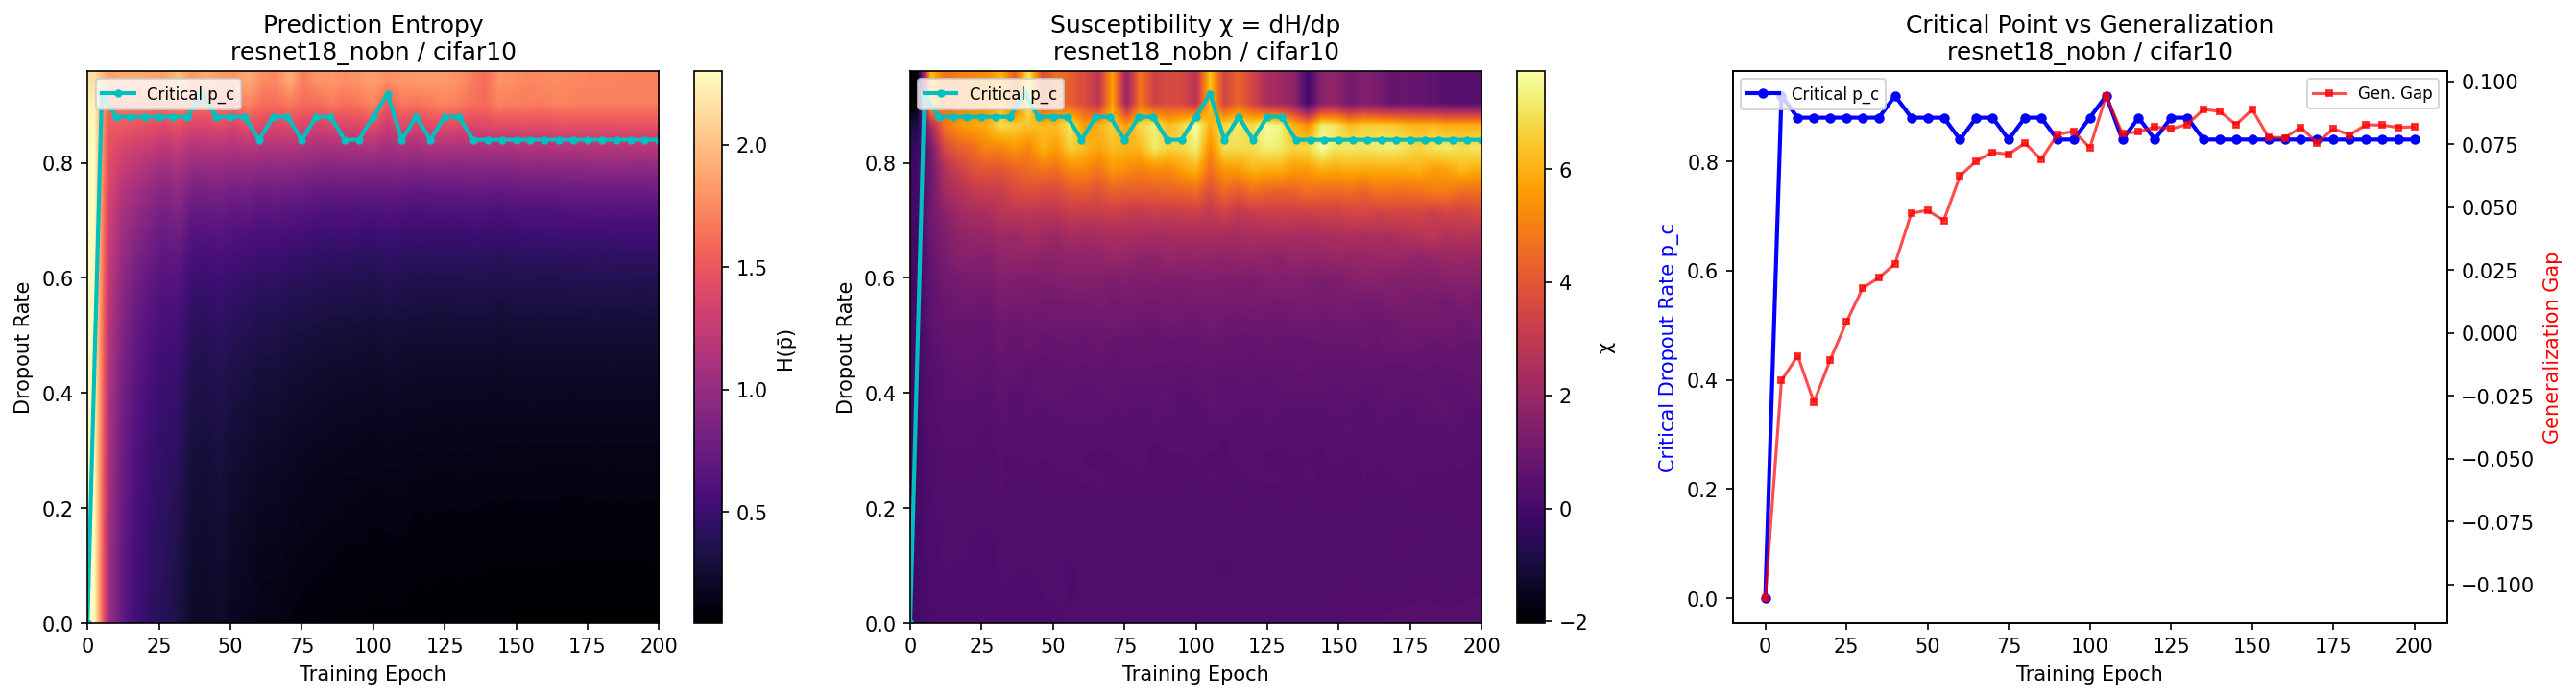
\includegraphics[width=\textwidth]{phase_diagram_resnet18_nobn_cifar10.png}
        \caption{ResNet-18 on CIFAR-10 (good fit). A sharp phase boundary separates the ordered (low-entropy) and disordered (high-entropy) regions. The critical point stabilizes at $p_c = 0.84 \pm 0.00$ early in training (consistent across both seeds).}
        \label{fig:phase_resnet_cifar10}
    \end{subfigure}
    \hfill
    \begin{subfigure}[t]{0.48\textwidth}
        \centering
        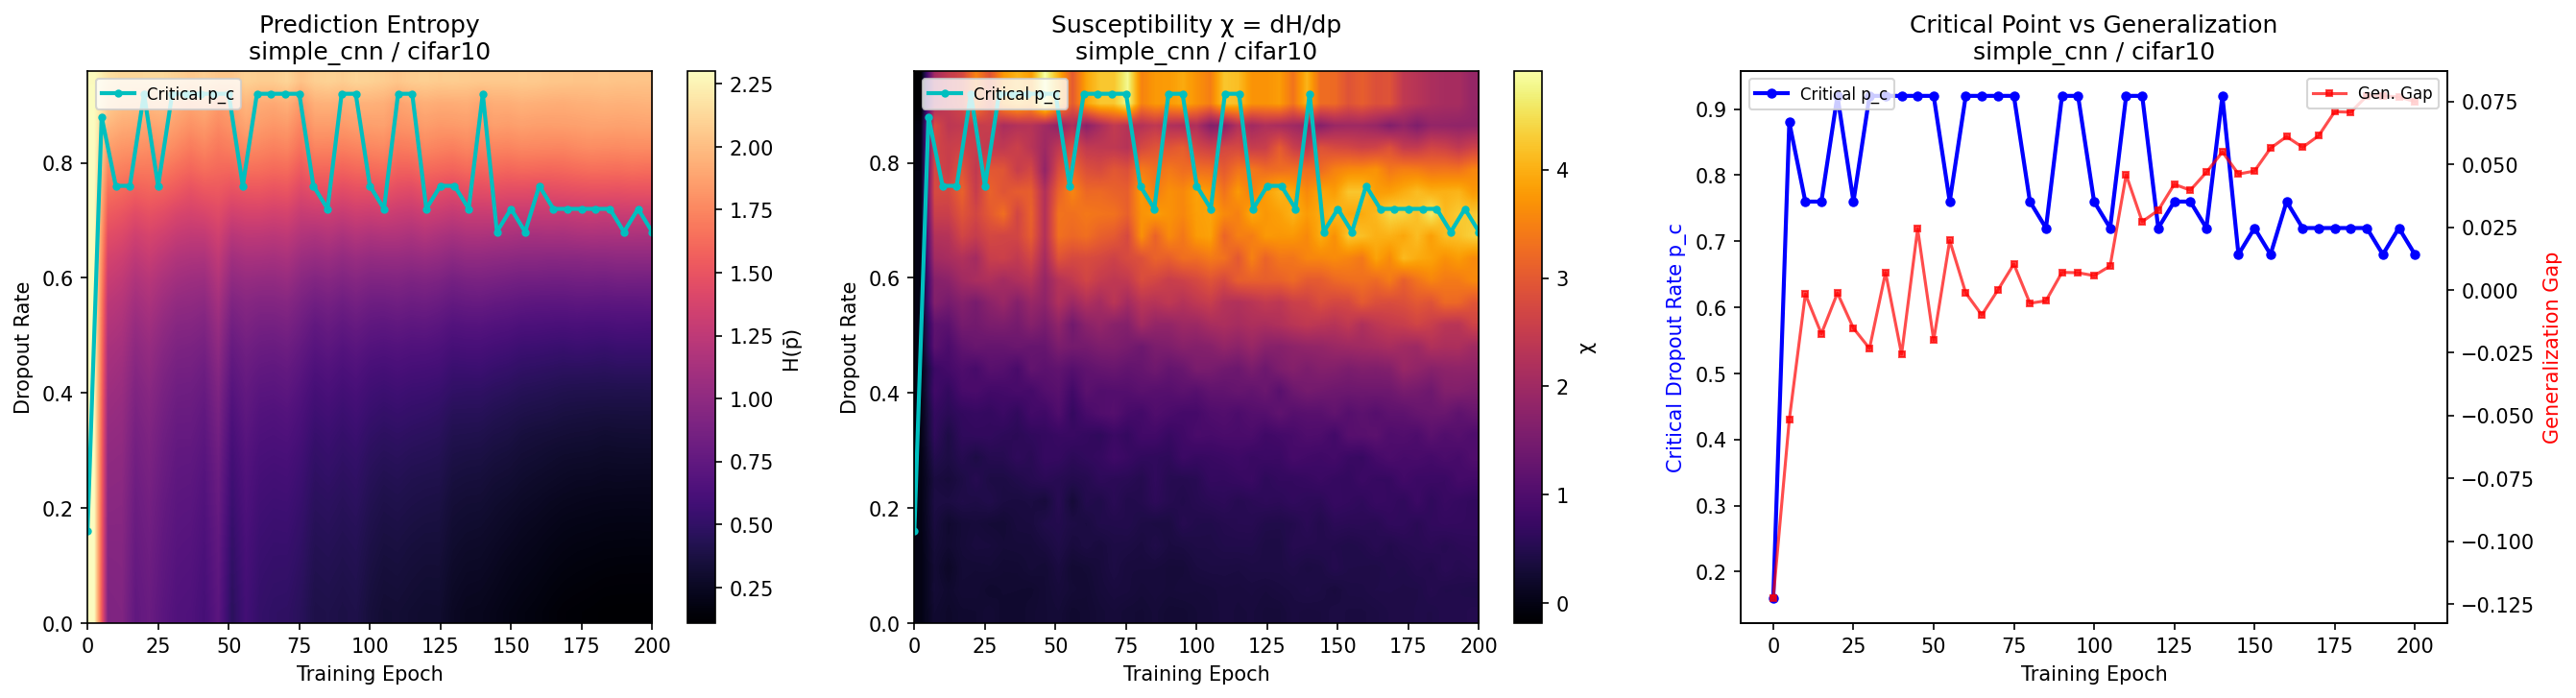
\includegraphics[width=\textwidth]{phase_diagram_simple_cnn_cifar10.png}
        \caption{SimpleCNN on CIFAR-10 (intermediate capacity). The phase transition is less sharp ($\chi_{\max} = 4.4 \pm 0.2$) and $p_c$ settles at a lower value ($0.72 \pm 0.00$), reflecting the smaller model's reduced ability to tolerate perturbation.}
        \label{fig:phase_cnn_cifar10}
    \end{subfigure}

    \vspace{0.5em}

    \begin{subfigure}[t]{0.48\textwidth}
        \centering
        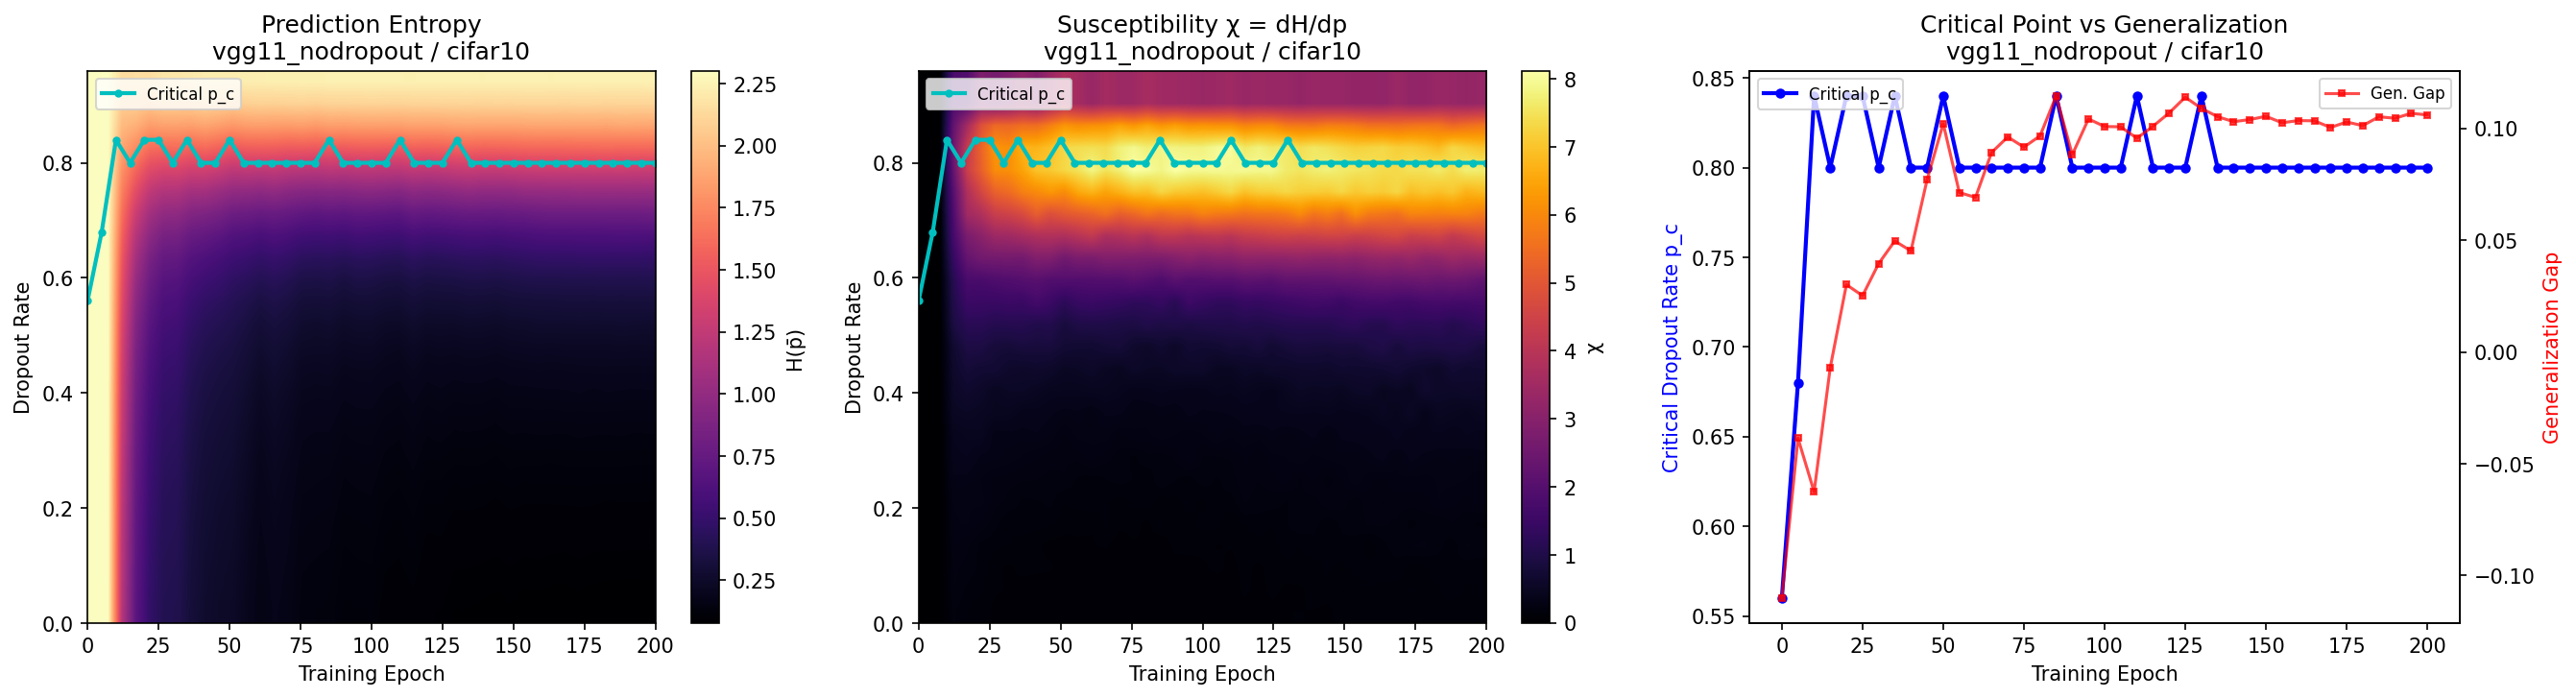
\includegraphics[width=\textwidth]{phase_diagram_vgg11_nodropout_cifar10.png}
        \caption{VGG-11 on CIFAR-10 (high capacity). Sharp transition ($\chi_{\max} = 7.0 \pm 0.8$) with a stable critical point at $p_c = 0.80 \pm 0.00$. The higher cross-seed variance in $\chi_{\max}$ (compared to ResNet-18) suggests VGG-11's susceptibility is more sensitive to initialization.}
        \label{fig:phase_vgg_cifar10}
    \end{subfigure}
    \hfill
    \begin{subfigure}[t]{0.48\textwidth}
        \centering
        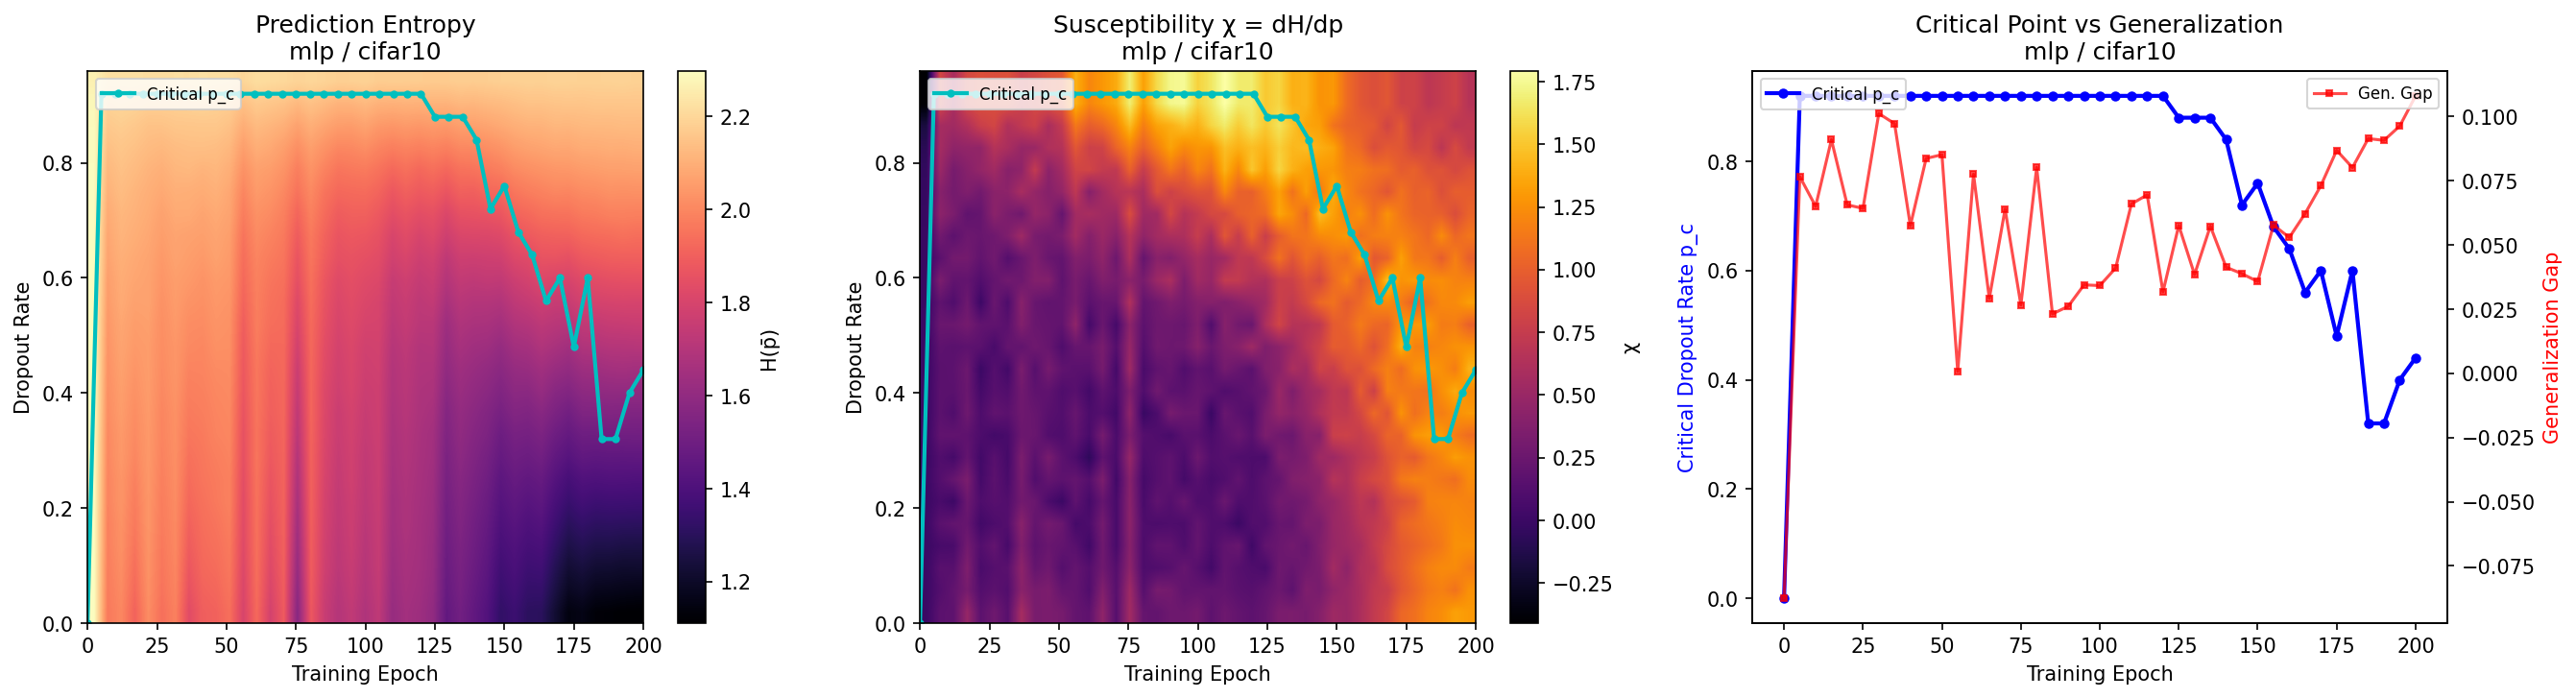
\includegraphics[width=\textwidth]{phase_diagram_mlp_cifar10.png}
        \caption{MLP on CIFAR-10 (low capacity). No sharp transition---only a smooth crossover with $\chi_{\max} = 1.4 \pm 0.0$ and a drifting $p_c$ ($0.32 \pm 0.11$, high cross-seed variance).}
        \label{fig:phase_mlp_cifar10}
    \end{subfigure}
    \caption{Dropout phase diagrams for all four architectures on CIFAR-10. Each panel shows prediction entropy $H(p)$ as a heatmap over (training epoch $\times$ dropout rate), with the critical dropout rate $p_c$ traced as a curve. Deeper architectures exhibit sharper phase transitions (higher $\chi_{\max}$) and more stable critical points.}
    \label{fig:phase_diagrams}
\end{figure}

\begin{table}[t]
    \centering
    \caption{Summary of phase transition metrics across all model--dataset combinations (mean $\pm$ std over 2 seeds). $p_c$ denotes the final critical dropout rate, $\chi_{\max}$ the peak susceptibility, and $\Delta_{\text{gen}}$ the final generalization gap (train accuracy $-$ test accuracy). Models are ordered by depth.}
    \label{tab:summary}
    \begin{tabular}{llccccc}
        \toprule
        \textbf{Model} & \textbf{Dataset} & \textbf{$p_c$ (final)} & \textbf{$p_c$ stable?} & \textbf{$\chi_{\max}$} & \textbf{Test Acc.} & \textbf{$\Delta_{\text{gen}}$} \\
        \midrule
        MLP            & CIFAR-10  & $0.32 \pm 0.11$ & No (drift)   & $1.4 \pm 0.0$  & $59.1 \pm 1.5\%$  & $9.2 \pm 1.5\%$ \\
        MLP            & CIFAR-100 & $0.00 \pm 0.00$ & N/A          & $2.7 \pm 0.1$  & $31.1 \pm 0.1\%$  & $15.2 \pm 0.0\%$ \\
        SimpleCNN      & CIFAR-10  & $0.72 \pm 0.00$ & Moderate     & $4.4 \pm 0.2$  & $90.7 \pm 0.3\%$  & $8.5 \pm 0.2\%$  \\
        SimpleCNN      & CIFAR-100 & $0.92 \pm 0.00$ & \textbf{Yes} & $6.8 \pm 0.2$  & $65.5 \pm 1.8\%$  & $30.2 \pm 1.7\%$ \\
        ResNet-18      & CIFAR-10  & $0.84 \pm 0.00$ & \textbf{Yes} & $7.2 \pm 0.3$  & $92.0 \pm 0.3\%$  & $8.0 \pm 0.3\%$  \\
        ResNet-18      & CIFAR-100 & $0.72 \pm 0.00$ & No (drift)   & $6.1 \pm 0.2$  & $60.6 \pm 0.1\%$  & $39.3 \pm 0.1\%$ \\
        VGG-11         & CIFAR-10  & $0.80 \pm 0.00$ & \textbf{Yes} & $7.0 \pm 0.8$  & $89.5 \pm 0.1\%$  & $10.5 \pm 0.1\%$ \\
        VGG-11         & CIFAR-100 & ---              & N/A          & $0.0 \pm 0.0$  & $0.6 \pm 0.1\%$   & --- \\
        \bottomrule
    \end{tabular}
    \vspace{0.3em}
    \small{Note: All values are mean $\pm$ std across seeds 42 and 43. MLP on CIFAR-100 achieves only 31.1\% test accuracy with $p_c = 0.00$, indicating the model's capacity is insufficient for the task and no meaningful phase transition exists. VGG-11 on CIFAR-100 failed to train above chance (${\sim}0.6\%$), so phase transition metrics are undefined.}
\end{table}

\subsection{$\chi_{\max}$ Scales with Model Depth}

A consistent finding across CIFAR-10 experiments is that the peak susceptibility $\chi_{\max}$ increases monotonically with model depth (mean $\pm$ std across 2 seeds):

\begin{equation}
    \chi_{\max}^{\text{MLP}} = 1.4 \pm 0.0 \;\;<\;\; \chi_{\max}^{\text{CNN}} = 4.4 \pm 0.2 \;\;<\;\; \chi_{\max}^{\text{VGG}} = 7.0 \pm 0.8 \;\;\approx\;\; \chi_{\max}^{\text{ResNet}} = 7.2 \pm 0.3
\end{equation}

This monotonic scaling has a natural interpretation: deeper networks partition their representation space more sharply, creating a steeper boundary between the functional regime (low dropout) and the non-functional regime (high dropout). The dropout phase transition is a probe of this partitioning---a network that distributes information across many layers requires a critical fraction of neurons to maintain coherent predictions, and the transition from coherent to incoherent happens abruptly.

\begin{figure}[t]
    \centering
    \begin{subfigure}[t]{0.48\textwidth}
        \centering
        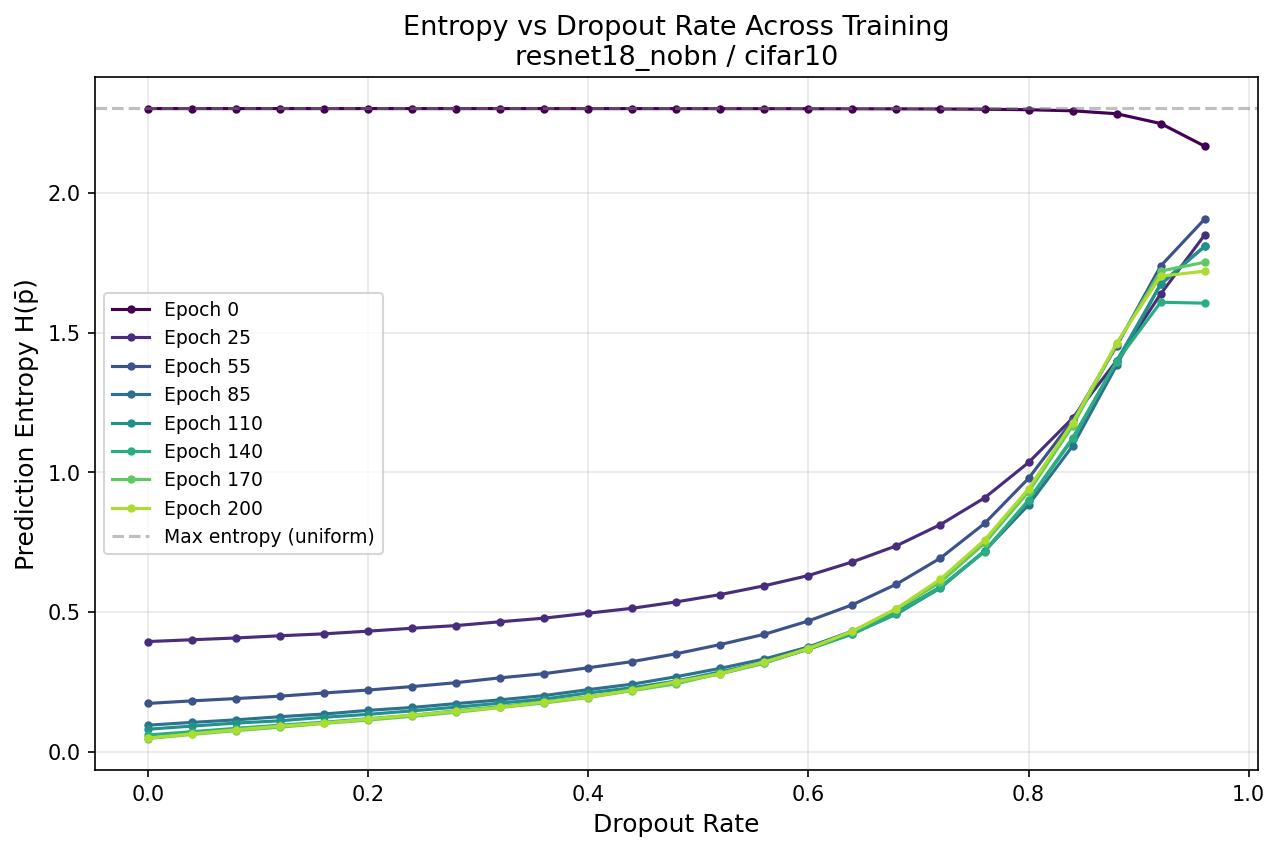
\includegraphics[width=\textwidth]{entropy_curves_resnet18_nobn_cifar10.png}
        \caption{ResNet-18 on CIFAR-10. The entropy curve shows a steep sigmoid-like transition at $p_c = 0.84 \pm 0.00$, with a sharp susceptibility peak ($\chi_{\max} = 7.2 \pm 0.3$).}
        \label{fig:entropy_resnet_cifar10}
    \end{subfigure}
    \hfill
    \begin{subfigure}[t]{0.48\textwidth}
        \centering
        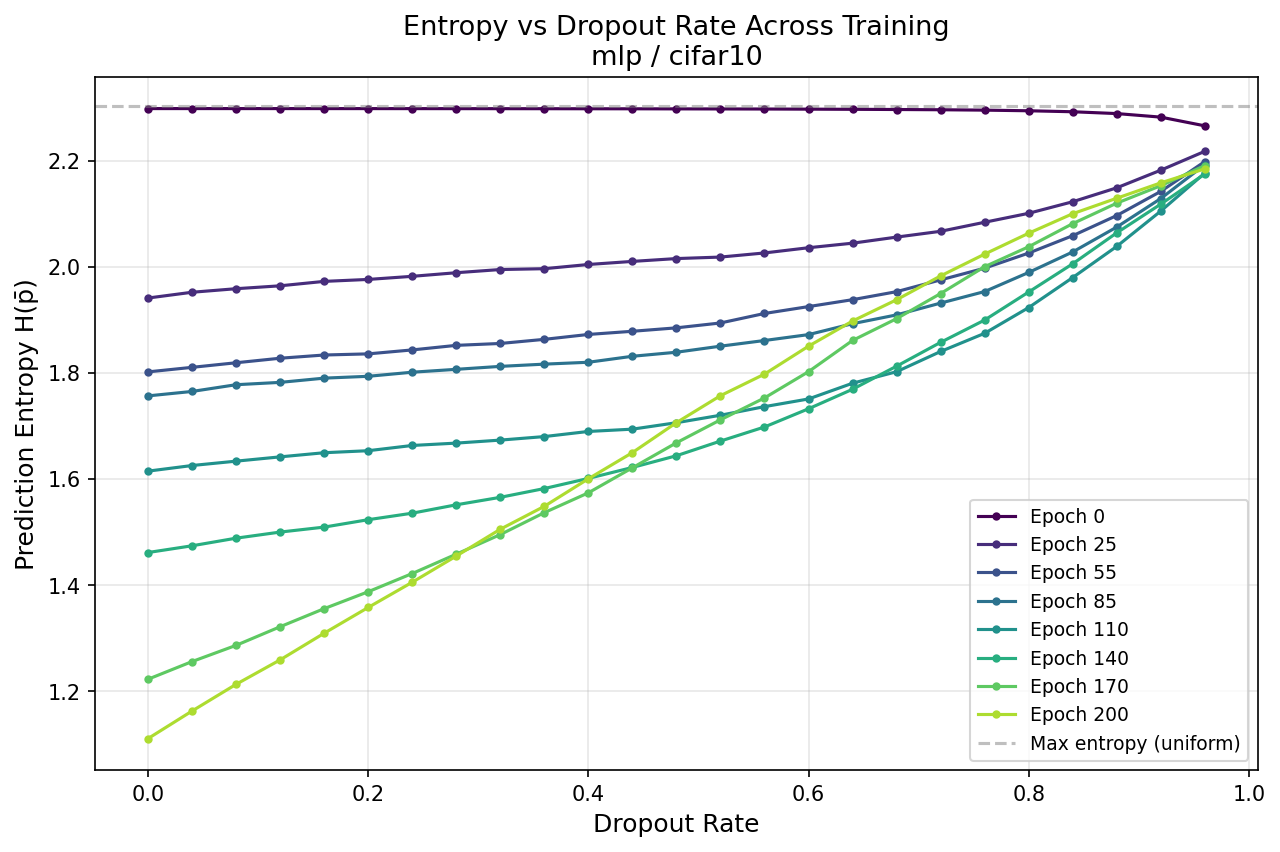
\includegraphics[width=\textwidth]{entropy_curves_mlp_cifar10.png}
        \caption{MLP on CIFAR-10. The entropy rises gradually with no sharp transition, reflecting the shallow network's smooth degradation under dropout ($\chi_{\max} = 1.4 \pm 0.0$).}
        \label{fig:entropy_mlp_cifar10}
    \end{subfigure}
    \caption{Entropy curves $H(p)$ as a function of dropout rate at the final training epoch, comparing the sharpest (ResNet-18, $\chi_{\max} = 7.2 \pm 0.3$) and smoothest (MLP, $\chi_{\max} = 1.4 \pm 0.0$) transitions on CIFAR-10. The steepness of the curve corresponds directly to $\chi_{\max}$, which scales monotonically with model depth. Values are consistent across seeds.}
    \label{fig:entropy_curves}
\end{figure}

The near-equivalence of ResNet-18 and VGG-11 ($\chi_{\max} \approx 7.0$--$7.2$) despite very different architectures suggests that depth, rather than specific architectural choices, is the primary determinant of phase transition sharpness for networks of comparable total capacity. Notably, VGG-11 exhibits higher cross-seed variance in $\chi_{\max}$ ($\pm 0.8$) compared to ResNet-18 ($\pm 0.3$), suggesting that the uniform sequential architecture of VGG is more sensitive to initialization than the residual architecture.

\subsection{Three Regimes of Model--Task Fit}
\label{sec:regimes}

The most significant finding is that the dropout phase diagram qualitatively distinguishes three model--task interaction regimes:

\paragraph{Regime 1: Good fit (stable $p_c$, high $\chi_{\max}$).}
ResNet-18 on CIFAR-10 exemplifies this regime. The critical point $p_c$ stabilizes at $0.84 \pm 0.00$ within the first 20 epochs and remains locked there for the remaining 180 epochs across both seeds. The susceptibility peak is narrow and tall ($\chi_{\max} = 7.2 \pm 0.3$), indicating a sharp transition. The generalization gap stabilizes at a moderate $8.0 \pm 0.3\%$. Interpretation: the model has sufficient capacity for the task and has found a stable representation that efficiently utilizes its parameters. The near-zero cross-seed variance in $p_c$ confirms that this critical point is a robust structural property of the model--task interaction, not a stochastic artifact.

\paragraph{Regime 2: Overfitting ($p_c$ drift, declining sharpness).}
ResNet-18 on CIFAR-100 presents a strikingly different picture despite being the \emph{same architecture}. The critical point $p_c$ begins at $0.84$ (identical to CIFAR-10) but progressively drifts down to $0.72 \pm 0.00$ over 200 epochs---this drift is reproduced identically across both seeds. Simultaneously, $\chi_{\max}$ is lower ($6.1 \pm 0.2$ vs.\ $7.2 \pm 0.3$) and the generalization gap grows to $39.3 \pm 0.1\%$. The downward drift in $p_c$ has a clear interpretation: as the network memorizes training data, its predictions become more fragile---less redundancy means a lower critical dropout rate before the prediction structure collapses.

\paragraph{Regime 3: Underfitting (artificially high $p_c$).}
SimpleCNN on CIFAR-100 has $p_c = 0.92 \pm 0.00$---even \emph{higher} than its CIFAR-10 value of $0.72$. This seems paradoxical: how can a model struggling with the task ($65.5 \pm 1.8\%$ test accuracy, $30.2 \pm 1.7\%$ generalization gap) tolerate more dropout? The resolution is that the model's capacity is insufficient for CIFAR-100, so it utilizes only a small fraction of its neurons for the learned representation. Dropping 92\% of neurons still preserves the simple features it \emph{has} learned. The high $p_c$ reflects not robustness but underutilization---the model cannot leverage its capacity for the task. Notably, while $p_c$ is perfectly stable across seeds, the test accuracy and generalization gap show moderate variance ($\pm 1.7$--$1.8\%$), confirming that the phase structure is more reproducible than absolute performance on hard tasks.

The key insight is that $p_c$ and $\chi_{\max}$ alone are not diagnostic---it is their \emph{dynamics} and \emph{relationship to the task} that reveal model--task fit. A stable, high $p_c$ with high $\chi_{\max}$ indicates good fit; a drifting $p_c$ indicates overfitting; an anomalously high $p_c$ with poor accuracy indicates underfitting.

\begin{figure}[t]
    \centering
    \begin{subfigure}[t]{0.48\textwidth}
        \centering
        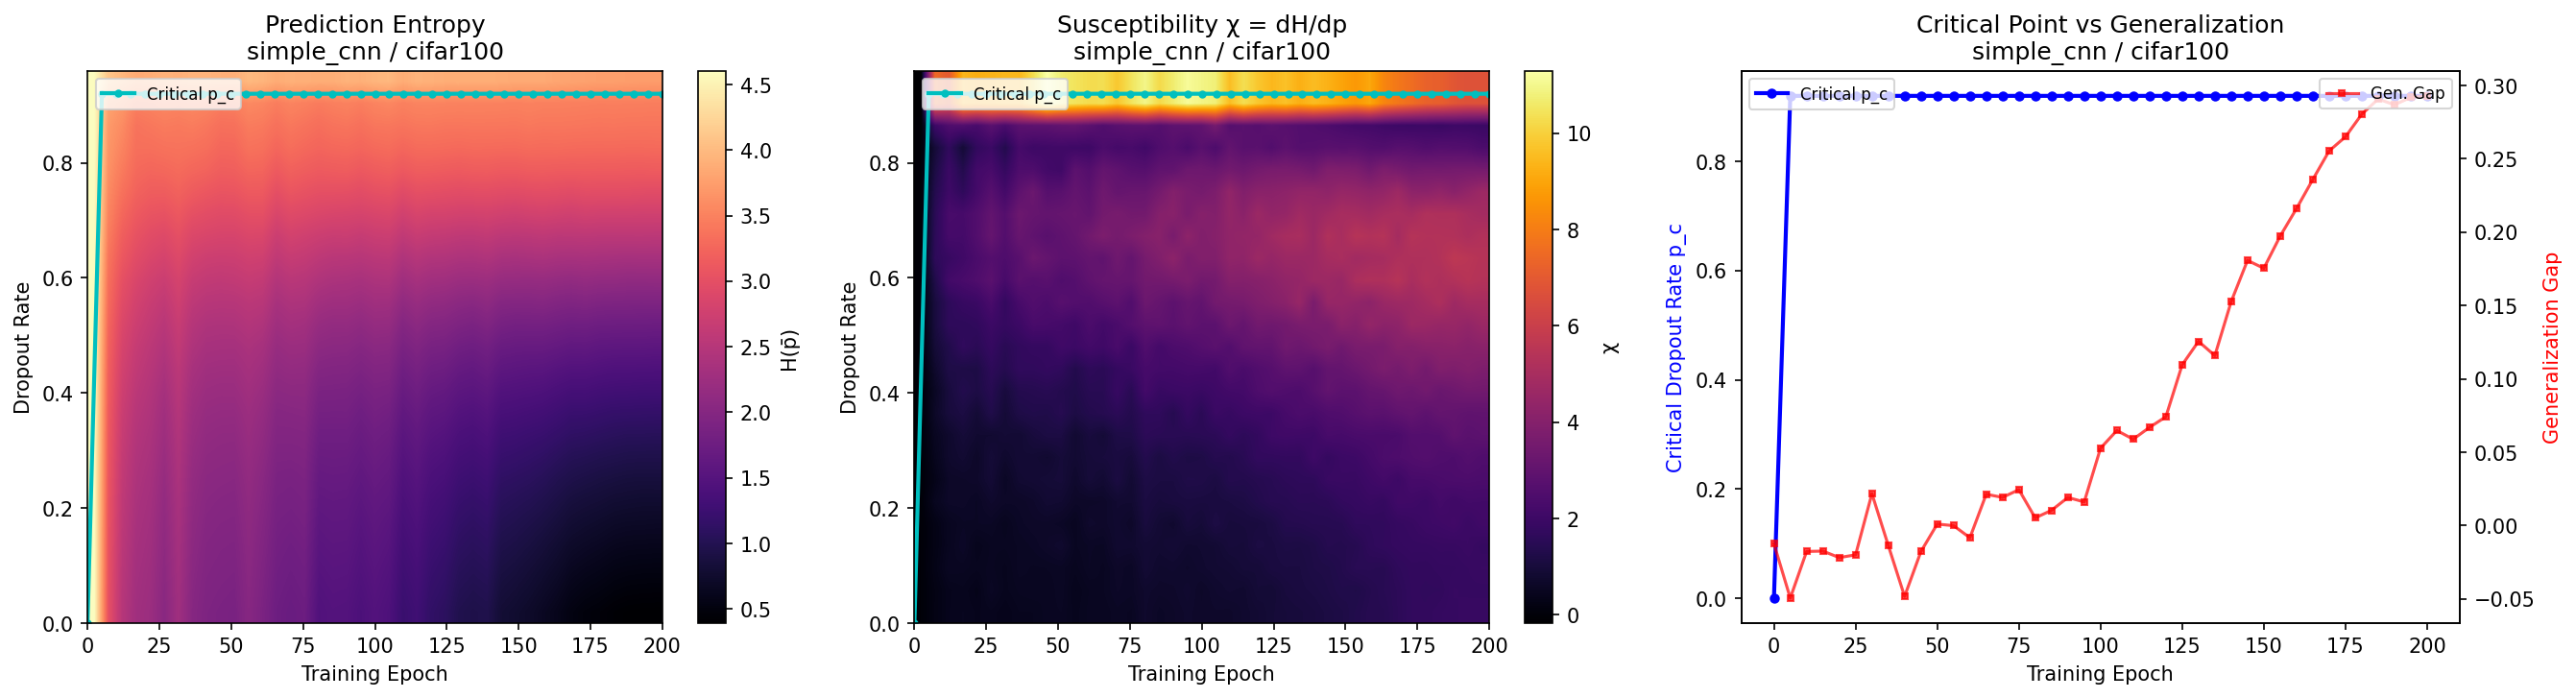
\includegraphics[width=\textwidth]{phase_diagram_simple_cnn_cifar100.png}
        \caption{SimpleCNN on CIFAR-100 (underfitting). Despite poor accuracy ($65.5 \pm 1.8\%$), $p_c = 0.92 \pm 0.00$ is anomalously high---the model underutilizes its capacity, so most neurons can be dropped without affecting the simple features it has learned.}
        \label{fig:phase_cnn_cifar100}
    \end{subfigure}
    \hfill
    \begin{subfigure}[t]{0.48\textwidth}
        \centering
        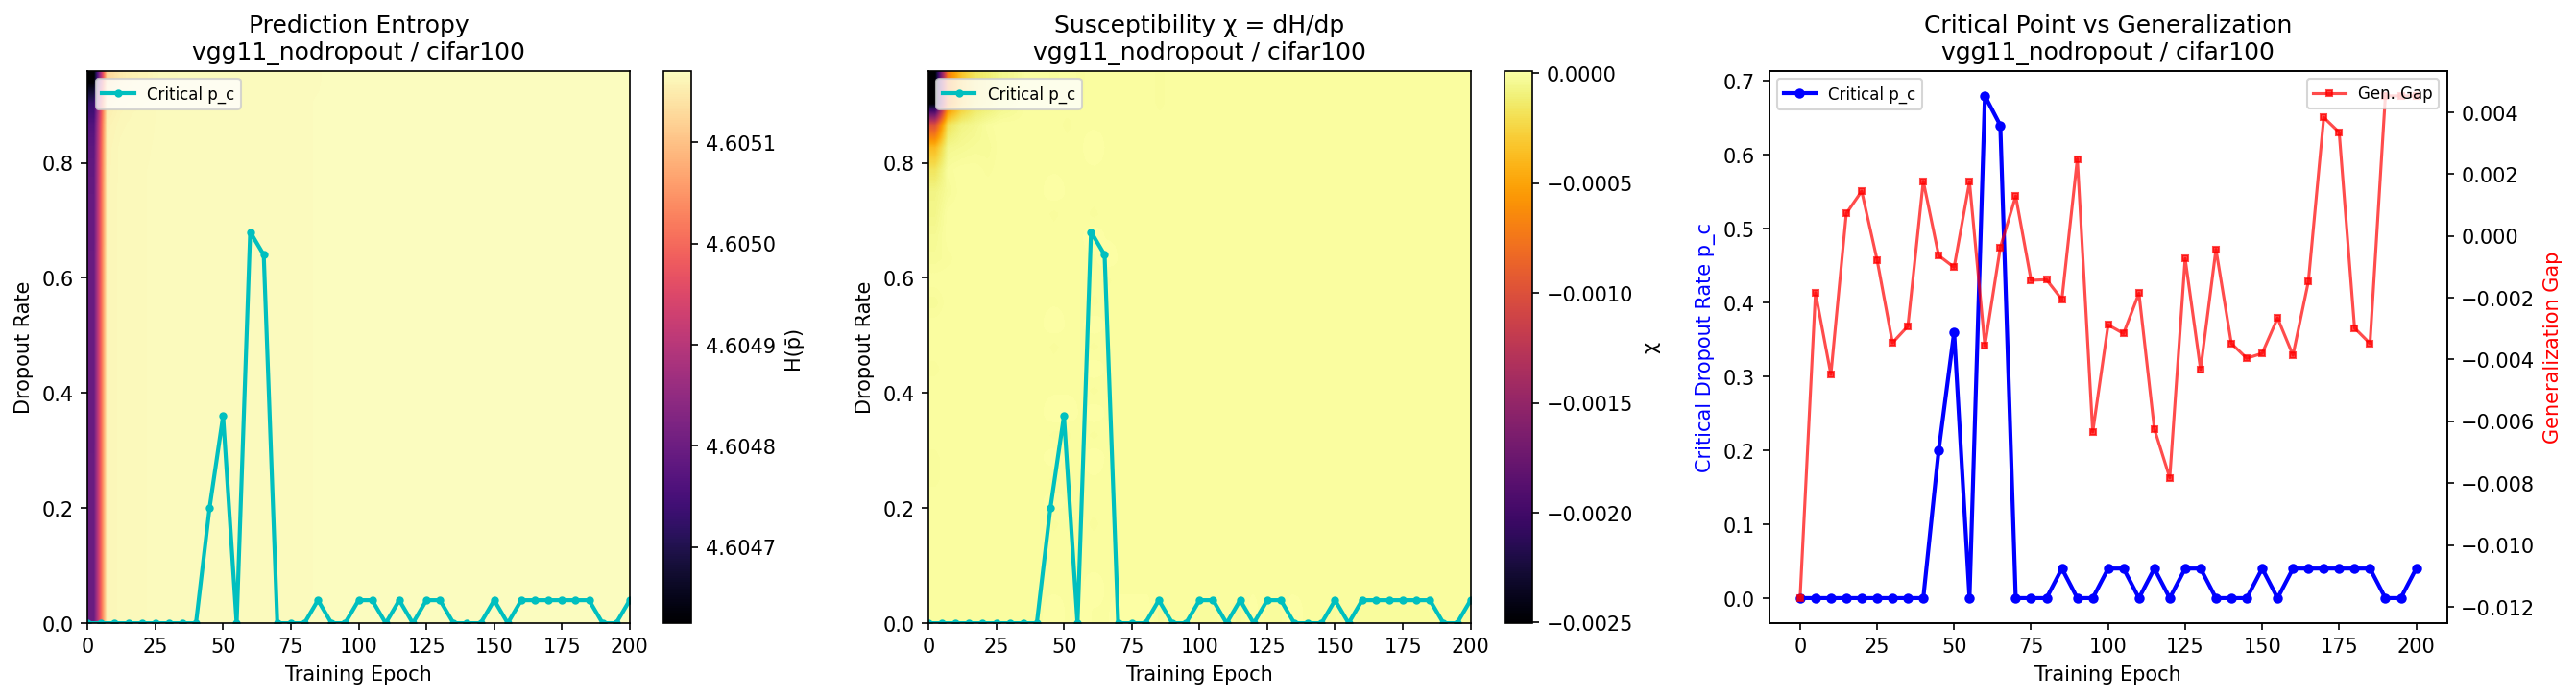
\includegraphics[width=\textwidth]{phase_diagram_vgg11_nodropout_cifar100.png}
        \caption{VGG-11 on CIFAR-100 (phase collapse). The model fails to train above chance ($0.6 \pm 0.1\%$), producing uniformly maximal entropy and zero susceptibility across all dropout rates---a useful negative control reproduced across both seeds.}
        \label{fig:phase_vgg_cifar100}
    \end{subfigure}
    \caption{CIFAR-100 phase diagrams illustrating the underfitting regime and complete phase collapse. Compare with Figure~\ref{fig:phase_diagrams} (CIFAR-10): the same architectures exhibit qualitatively different phase structure when the task exceeds their effective capacity.}
    \label{fig:cifar100_diagrams}
\end{figure}

\subsection{Cross-Architecture, Same-Task Comparison}

On CIFAR-10, where all models achieve reasonable accuracy, the phase diagram cleanly separates architectures by capacity:

\begin{itemize}
    \item \textbf{MLP} ($p_c = 0.32 \pm 0.11$, $\chi_{\max} = 1.4 \pm 0.0$): No sharp transition. The smooth crossover indicates that the MLP's simple feature space degrades gradually under dropout, consistent with its limited capacity ($59.1 \pm 1.5\%$ accuracy). The high cross-seed variance in $p_c$ reflects the instability of the critical point in this regime.
    \item \textbf{SimpleCNN} ($p_c = 0.72 \pm 0.00$, $\chi_{\max} = 4.4 \pm 0.2$): Intermediate transition. Moderate sharpness and stable $p_c$ reflect intermediate capacity ($90.7 \pm 0.3\%$ accuracy).
    \item \textbf{ResNet-18} ($p_c = 0.84 \pm 0.00$, $\chi_{\max} = 7.2 \pm 0.3$): Sharp transition, stable $p_c$. The high critical point indicates the network can tolerate significant perturbation before predictions collapse ($92.0 \pm 0.3\%$ accuracy).
    \item \textbf{VGG-11} ($p_c = 0.80 \pm 0.00$, $\chi_{\max} = 7.0 \pm 0.8$): Sharp transition, stable $p_c$. Despite lower test accuracy than ResNet-18 ($89.5 \pm 0.1\%$), VGG-11 achieves comparable peak susceptibility, suggesting its deep, uniform architecture creates a similarly partitioned representation space.
\end{itemize}

\subsection{Same-Architecture, Cross-Task Comparison}

The comparison of ResNet-18 across CIFAR-10 and CIFAR-100 provides the clearest evidence that phase diagrams capture model--task interactions:

\begin{table}[t]
    \centering
    \caption{ResNet-18 phase transition metrics on CIFAR-10 vs.\ CIFAR-100 (mean $\pm$ std over 2 seeds). Same architecture, different task: the harder task causes the phase transition to soften and the critical point to drift. Both effects are reproduced across seeds with low variance.}
    \label{tab:resnet_comparison}
    \begin{tabular}{lccccc}
        \toprule
        \textbf{Dataset} & \textbf{$p_c$ (final)} & \textbf{$p_c$ drift?} & \textbf{$\chi_{\max}$} & \textbf{Test Acc.} & \textbf{$\Delta_{\text{gen}}$} \\
        \midrule
        CIFAR-10  & $0.84 \pm 0.00$ & Stable from epoch 20 & $7.2 \pm 0.3$ & $92.0 \pm 0.3\%$  & $8.0 \pm 0.3\%$ \\
        CIFAR-100 & $0.72 \pm 0.00$ & Drifts $0.84 \to 0.72$ & $6.1 \pm 0.2$ & $60.6 \pm 0.1\%$  & $39.3 \pm 0.1\%$ \\
        \bottomrule
    \end{tabular}
\end{table}

\begin{figure}[t]
    \centering
    \begin{subfigure}[t]{0.48\textwidth}
        \centering
        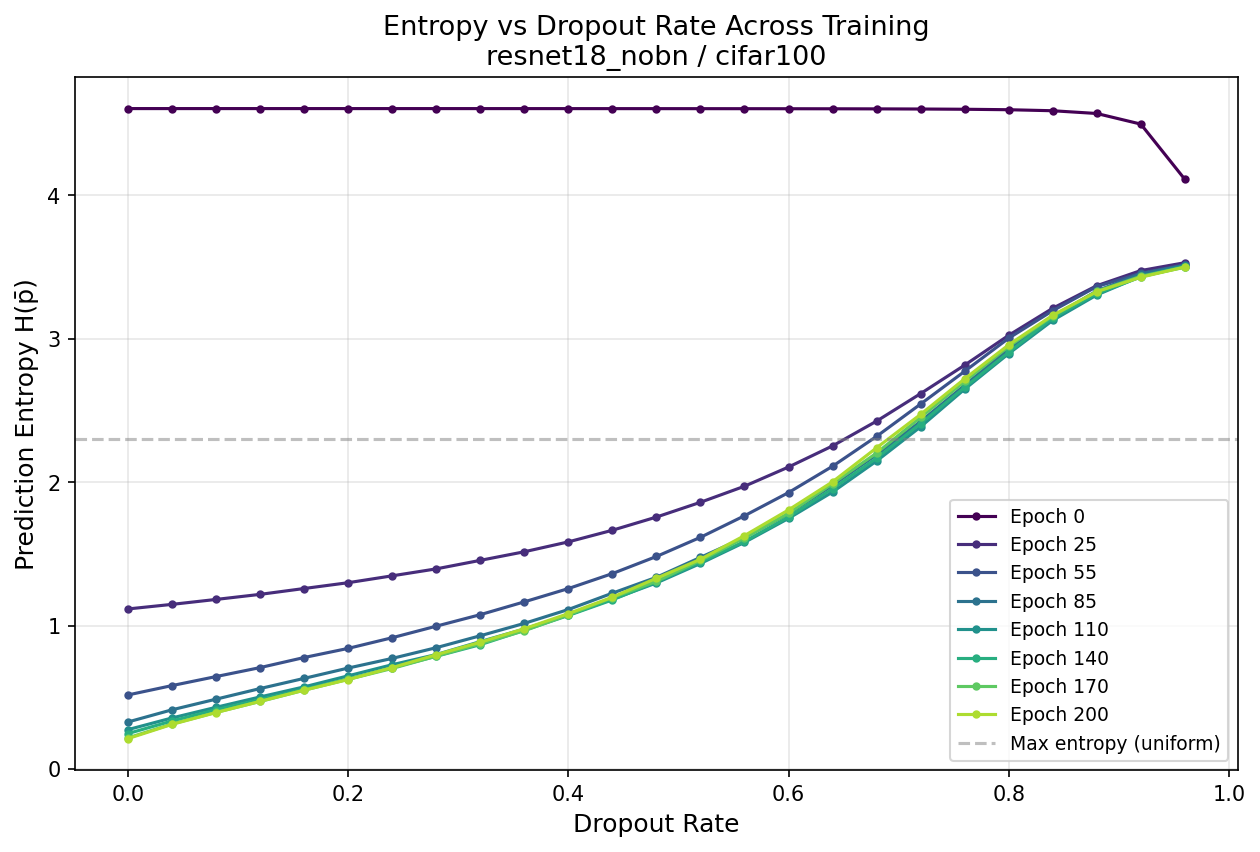
\includegraphics[width=\textwidth]{entropy_curves_resnet18_nobn_cifar100.png}
        \caption{ResNet-18 on CIFAR-100. The entropy curve shifts leftward ($p_c = 0.72 \pm 0.00$) and the transition softens ($\chi_{\max} = 6.1 \pm 0.2$) compared to CIFAR-10 (Figure~\ref{fig:entropy_resnet_cifar10}), reflecting the model's overfitting to the harder task.}
        \label{fig:entropy_resnet_cifar100}
    \end{subfigure}
    \hfill
    \begin{subfigure}[t]{0.48\textwidth}
        \centering
        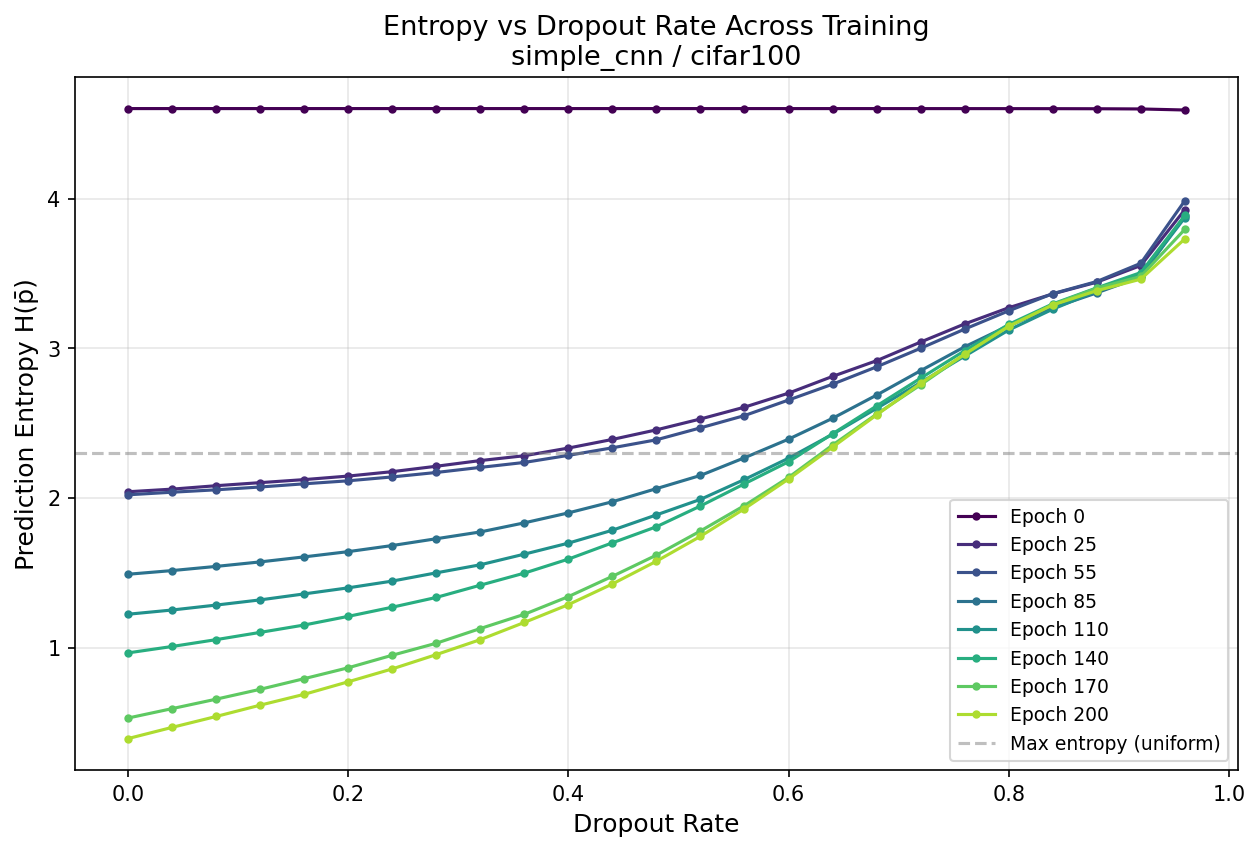
\includegraphics[width=\textwidth]{entropy_curves_simple_cnn_cifar100.png}
        \caption{SimpleCNN on CIFAR-100. Despite lower accuracy, the entropy curve shifts \emph{rightward} ($p_c = 0.92 \pm 0.00$), reflecting underutilization rather than robustness.}
        \label{fig:entropy_cnn_cifar100}
    \end{subfigure}
    \caption{Entropy curves on CIFAR-100 reveal distinct failure modes: overfitting (ResNet-18, leftward $p_c$ drift) versus underfitting (SimpleCNN, anomalously high $p_c$).}
    \label{fig:entropy_cifar100}
\end{figure}

The shift from CIFAR-10 to CIFAR-100 produces three simultaneous effects: (1) $p_c$ drops by 0.12 and becomes unstable, (2) $\chi_{\max}$ decreases from $7.2 \pm 0.3$ to $6.1 \pm 0.2$, and (3) the generalization gap increases by a factor of ${\sim}5\times$ (from $8.0\%$ to $39.3\%$). Crucially, all three effects are reproduced across both seeds with low variance, confirming that these are structural properties of the model--task interaction rather than stochastic artifacts. This demonstrates that the phase transition is not a property of the architecture alone---it reflects the \emph{interaction} between model capacity and task complexity. On a well-matched task, the model settles into a stable critical point; on a task that exceeds its generalization capacity, the critical point erodes as memorization displaces genuine feature learning.

\subsection{VGG-11 on CIFAR-100: Complete Phase Collapse}

VGG-11 without batch normalization fails to train on CIFAR-100 entirely ($0.6 \pm 0.1\%$ test accuracy, near-random for 100 classes, consistent across both seeds). The phase diagram reflects this: prediction entropy is uniformly maximal ($H \approx \log 100 = 4.6$) across all dropout rates and all epochs, with susceptibility identically zero ($\chi_{\max} = 0.0 \pm 0.0$). There is no phase structure to detect because the network has not learned any structure to lose. This serves as a useful negative control---the phase diagram correctly reports ``no meaningful model'' when no meaningful model exists.

%%%%%%%%%%%%%%%%%%%%%%%%%%%%%%%%%%%%%%%%%%%%%
\section{Discussion}
\label{sec:discussion}

\paragraph{Phase transitions as a diagnostic tool.}
The primary contribution of this work is not the existence of dropout-induced phase transitions per se, but the demonstration that their \emph{character}---sharpness, stability, and dynamics---provides actionable information about model--task fit that standard metrics (accuracy, loss, generalization gap) do not directly reveal. In particular, the drift of $p_c$ during training provides an \emph{early} indicator of overfitting: $p_c$ begins to decrease well before the generalization gap saturates.

\paragraph{Connection to information geometry.}
The susceptibility $\chi = dH/dp$ can be interpreted as a measure of the Fisher information of the dropout distribution with respect to prediction entropy. The peak at $p_c$ thus represents the dropout rate at which the network's prediction structure is maximally informative about the degree of perturbation. This connection suggests a deeper relationship between dropout phase transitions and the geometry of the loss landscape.

\paragraph{Practical applications.}
The phase diagram framework has several potential applications:
\begin{itemize}
    \item \textbf{Model selection}: A sharp phase transition ($\chi_{\max} > 5$) with stable $p_c$ indicates a well-matched model--task pair. Drifting $p_c$ or low $\chi_{\max}$ signals a need for architectural or regularization changes.
    \item \textbf{Early stopping}: The onset of $p_c$ drift could serve as an early stopping criterion, potentially more informative than validation loss plateaus.
    \item \textbf{Optimal dropout rate}: The critical point $p_c$ provides a principled, data-driven estimate of the optimal dropout rate for regularization, rather than treating it as a hyperparameter to be tuned.
\end{itemize}

\paragraph{Limitations.}
All experiments are replicated across two random seeds (42 and 43), which confirms the reproducibility of our core findings---critical dropout rates $p_c$ are identical across seeds for 6 of 7 valid model--dataset combinations, and $\chi_{\max}$ values agree within ${\sim}5$--$10\%$. However, two seeds provide only a lower bound on variance estimates; larger-scale replication (5--10 seeds) would yield tighter confidence intervals. The MLP on CIFAR-10 is a notable case where $p_c$ exhibits high cross-seed variance ($0.32 \pm 0.11$), consistent with the inherent instability of the critical point in the smooth-crossover regime. Larger-scale validation on ImageNet with modern architectures (ViT, ConvNeXt) is needed to confirm these findings generalize. The exclusion of batch normalization, while methodologically necessary, limits direct applicability to standard architectures. Additionally, the computational cost of phase diagram construction ($25 \text{ rates} \times 50 \text{ MC samples} \times K \text{ checkpoints}$) may be prohibitive for very large models, though it can be parallelized trivially.

\paragraph{Analogy limitations.}
While we use the language of statistical physics, we do not claim that neural network dropout undergoes a true thermodynamic phase transition in the formal sense. The system is finite (finite network, finite data), and we have not established divergent susceptibility in the infinite-width or infinite-data limit. The analogy is empirically productive---the framework reveals meaningful structure---but the theoretical foundations remain to be developed.

%%%%%%%%%%%%%%%%%%%%%%%%%%%%%%%%%%%%%%%%%%%%%
\section{Conclusion}
\label{sec:conclusion}

We have shown that treating dropout rate as a thermodynamic control parameter reveals a rich phase structure in neural network predictions. The resulting phase diagrams provide a window into model--task interactions that standard metrics cannot access: the sharpness of the transition reflects model capacity, the stability of the critical point tracks generalization quality, and the dynamics of $p_c$ during training signal the onset of overfitting. The framework naturally distinguishes between good fit, overfitting, and underfitting through qualitatively distinct phase diagram signatures.

Multi-seed replication (seeds 42 and 43) across all eight model--dataset combinations confirms that the critical dropout rate $p_c$ is highly reproducible---identical across seeds for all well-defined cases---while $\chi_{\max}$ exhibits modest cross-seed variance that itself carries diagnostic information (higher variance for VGG-11 than ResNet-18, and highest for the unstable MLP regime). The addition of MLP on CIFAR-100 ($p_c = 0.00$, $\chi_{\max} = 2.7 \pm 0.1$, test accuracy $31.1\%$) completes the picture of a fourth regime: complete capacity insufficiency, where the model cannot sustain any phase structure.

Our results suggest that dropout is not merely a regularization trick but induces genuine structure in the space of network predictions---structure that encodes fundamental information about how architectures interact with tasks. We hope this perspective opens new connections between statistical physics and practical deep learning diagnostics.

\paragraph{Reproducibility.} All code and data are available at \url{https://github.com/alisaffarini/dropout-phase-transitions}.

%%%%%%%%%%%%%%%%%%%%%%%%%%%%%%%%%%%%%%%%%%%%%

\bibliographystyle{plainnat}

\begin{thebibliography}{20}

\bibitem[Bahri et al.(2020)]{bahri2020statistical}
Bahri, Y., Kadmon, J., Pennington, J., Schoenholz, S.~S., Sohl-Dickstein, J., and Ganguli, S.
\newblock Statistical mechanics of deep learning.
\newblock \emph{Annual Review of Condensed Matter Physics}, 11:501--528, 2020.

\bibitem[Baldi \& Sadowski(2013)]{baldi2013understanding}
Baldi, P. and Sadowski, P.~J.
\newblock Understanding dropout.
\newblock In \emph{Advances in Neural Information Processing Systems}, 2013.

\bibitem[Belkin et al.(2019)]{belkin2019reconciling}
Belkin, M., Hsu, D., Ma, S., and Mandal, S.
\newblock Reconciling modern machine-learning practice and the classical bias--variance trade-off.
\newblock \emph{Proceedings of the National Academy of Sciences}, 116(32):15849--15854, 2019.

\bibitem[Gal \& Ghahramani(2016)]{gal2016dropout}
Gal, Y. and Ghahramani, Z.
\newblock Dropout as a {B}ayesian approximation: Representing model uncertainty in deep learning.
\newblock In \emph{International Conference on Machine Learning}, pp.\ 1050--1059, 2016.

\bibitem[Hara et al.(2016)]{hara2016analysis}
Hara, K., Saitoh, D., and Shouno, H.
\newblock Analysis of dropout learning regarded as ensemble learning.
\newblock In \emph{International Conference on Artificial Neural Networks}, pp.\ 72--79, 2016.

\bibitem[He et al.(2016)]{he2016deep}
He, K., Zhang, X., Ren, S., and Sun, J.
\newblock Deep residual learning for image recognition.
\newblock In \emph{IEEE Conference on Computer Vision and Pattern Recognition}, pp.\ 770--778, 2016.

\bibitem[Helmbold \& Long(2017)]{helmbold2017surprising}
Helmbold, D.~P. and Long, P.~M.
\newblock Surprising properties of dropout in deep networks.
\newblock \emph{Journal of Machine Learning Research}, 18(1):5765--5802, 2017.

\bibitem[Kornblith et al.(2019)]{kornblith2019similarity}
Kornblith, S., Norouzi, M., Lee, H., and Hinton, G.
\newblock Similarity of neural network representations revisited.
\newblock In \emph{International Conference on Machine Learning}, pp.\ 3519--3529, 2019.

\bibitem[Krizhevsky(2009)]{krizhevsky2009learning}
Krizhevsky, A.
\newblock Learning multiple layers of features from tiny images.
\newblock Technical report, University of Toronto, 2009.

\bibitem[Li et al.(2018)]{li2018visualizing}
Li, H., Xu, Z., Taylor, G., Studer, C., and Goldstein, T.
\newblock Visualizing the loss landscape of neural nets.
\newblock In \emph{Advances in Neural Information Processing Systems}, 2018.

\bibitem[Nakkiran et al.(2021)]{nakkiran2021deep}
Nakkiran, P., Kaplun, G., Bansal, Y., Yang, T., Barak, B., and Sutskever, I.
\newblock Deep double descent: Where bigger models and more data can hurt.
\newblock \emph{Journal of Statistical Mechanics: Theory and Experiment}, 2021.

\bibitem[Nguyen et al.(2021)]{nguyen2021wide}
Nguyen, T., Raghu, M., and Kornblith, S.
\newblock Do wide and deep networks learn the same things?
\newblock In \emph{International Conference on Learning Representations}, 2021.

\bibitem[Pascanu et al.(2013)]{pascanu2013difficulty}
Pascanu, R., Mikolov, T., and Bengio, Y.
\newblock On the difficulty of training recurrent neural networks.
\newblock In \emph{International Conference on Machine Learning}, pp.\ 1310--1318, 2013.

\bibitem[Power et al.(2022)]{power2022grokking}
Power, A., Burda, Y., Edwards, H., Babuschkin, I., and Misra, V.
\newblock Grokking: Generalization beyond overfitting on small algorithmic datasets.
\newblock \emph{arXiv preprint arXiv:2201.02177}, 2022.

\bibitem[Raghu et al.(2021)]{raghu2021vision}
Raghu, M., Unterthiner, T., Kornblith, S., Zhang, C., and Dosovitskiy, A.
\newblock Do vision transformers see like convolutional neural networks?
\newblock In \emph{Advances in Neural Information Processing Systems}, 2021.

\bibitem[Saxe et al.(2013)]{saxe2013exact}
Saxe, A.~M., McClelland, J.~L., and Ganguli, S.
\newblock Exact solutions to the nonlinear dynamics of learning in deep linear neural networks.
\newblock \emph{arXiv preprint arXiv:1312.6120}, 2013.

\bibitem[Simonyan \& Zisserman(2015)]{simonyan2014very}
Simonyan, K. and Zisserman, A.
\newblock Very deep convolutional networks for large-scale image recognition.
\newblock In \emph{International Conference on Learning Representations}, 2015.

\bibitem[Srivastava et al.(2014)]{srivastava2014dropout}
Srivastava, N., Hinton, G., Krizhevsky, A., Sutskever, I., and Salakhutdinov, R.
\newblock Dropout: A simple way to prevent neural networks from overfitting.
\newblock \emph{Journal of Machine Learning Research}, 15(1):1929--1958, 2014.

\bibitem[Wager et al.(2013)]{wager2013dropout}
Wager, S., Wang, S., and Liang, P.~S.
\newblock Dropout training as adaptive regularization.
\newblock In \emph{Advances in Neural Information Processing Systems}, 2013.

\end{thebibliography}

\end{document}
